% ============================================================
% 1. Introduction -- the two original frames from main.tex.
% ============================================================
\section{Introduction}

\setsource{}
\begin{frame}[label=intro-1]{Introduction: Why AI?}
\small

 Nuclear astrophysics is suitable for AI due to some characteristics.

\vspace{0.2cm}

\begin{itemize}
\setlength{\itemsep}{0.6em}

    \item \textbf{Interdisciplinary with Knowledge Gaps}

    Relevant knowledge is distributed across nuclear physics, astrophysics, and observational literature.
    
    \item \textbf{Simulation-Based \& Computationally Constrained}

    Full nucleosynthesis simulations may involve \(\sim10^3\) isotopes and up to \(\sim10^4\) reactions, coupling with 2D/3D hydrodynamics.
    
    \item \textbf{Experimentally Expensive}

    Experiments involve many coupled setup parameters, while beam time and machine access are limited and costly.
    

    \item \textbf{Uncertainty-Sensitivity Intensive}

    Make predictions and identify which uncertain inputs dominate the results should be prioritized for theory and experiments.
    

\end{itemize}

\end{frame}

%

\setsource{}
\begin{frame}[label=intro-2]{Introduction: ML in Nuc/Astro}

Machine learning has already been widely explored in both nuclear physics
and astrophysics.

\vspace{0.15cm}

\centering
\resizebox{\textwidth}{!}{%
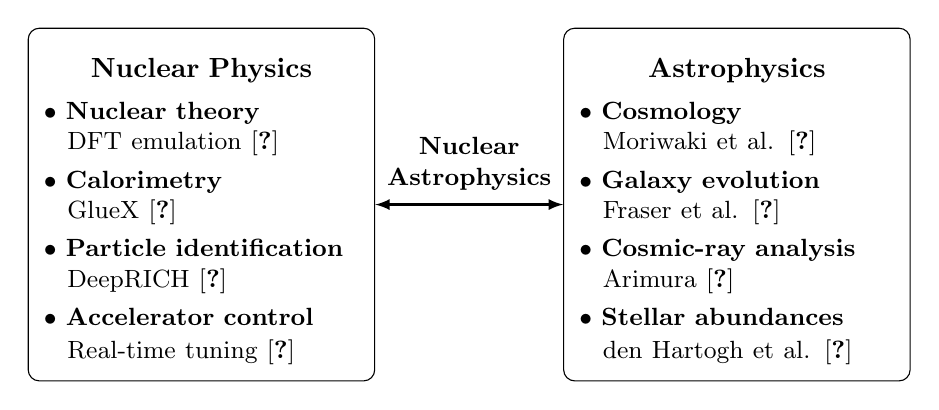
\begin{tikzpicture}[>=latex]

\node[
    draw,
    rounded corners,
    align=left,
    text width=4.0cm,
    minimum height=3.55cm,
    inner sep=0.20cm
] (nuc) at (-3.4,0) {

    \centering
    \textbf{Nuclear Physics}

    \vspace{0.15cm}
    \raggedright
    \small

    $\bullet$ \textbf{Nuclear theory}\\
    \hspace{0.18cm} DFT emulation \cite{lasseri2020}

    \vspace{0.10cm}

    $\bullet$ \textbf{Calorimetry}\\
    \hspace{0.18cm} GlueX \cite{barsotti2020}

    \vspace{0.10cm}

    $\bullet$ \textbf{Particle identification}\\
    \hspace{0.18cm} DeepRICH \cite{fanelli2020}

    \vspace{0.10cm}

    $\bullet$ \textbf{Accelerator control}\\
    \hspace{0.18cm} Real-time tuning \cite{scheinker2019}
};

\node[
    draw,
    rounded corners,
    align=left,
    text width=4.0cm,
    minimum height=3.55cm,
    inner sep=0.20cm
] (astro) at (3.4,0) {

    \centering
    \textbf{Astrophysics}

    \vspace{0.15cm}
    \raggedright
    \small

    $\bullet$ \textbf{Cosmology}\\
    \hspace{0.18cm} Moriwaki et al. \cite{moriwaki2023}

    \vspace{0.10cm}

    $\bullet$ \textbf{Galaxy evolution}\\
    \hspace{0.18cm} Fraser et al. \cite{fraser2023}

    \vspace{0.10cm}

    $\bullet$ \textbf{Cosmic-ray analysis}\\
    \hspace{0.18cm} Arimura \cite{arimura2023}

    \vspace{0.10cm}

    $\bullet$ \textbf{Stellar abundances}\\
    \hspace{0.18cm} den Hartogh et al. \cite{denhartogh2023}
};

\draw[<->, thick]
    (nuc.east) --
    node[
        above,
        midway,
        align=center,
        yshift=0.05cm
    ] {
        \small\textbf{Nuclear}\\[-0.03cm]
        \small\textbf{Astrophysics}
    }
    (astro.west);

\end{tikzpicture}}

\vspace{0.03cm}

\begin{flushleft}
{
However, while ML has advanced both fields separately, its use in nuclear astrophysics remains very limited \cite{smith2024}.
}
\end{flushleft}


\note{\begin{description}
\item[1] R. Lasseri, D. Regnier, J. Ebran, and A. Penon,
``Taming Nuclear Complexity with a Committee of Multilayer Neural Networks,''
\textit{Phys. Rev. Lett.} \textbf{124}, 162502 (2020).
\item[2] R. Barsotti and M. R. Shepherd,
``Using machine learning to separate hadronic and electromagnetic interactions
in the GlueX forward calorimeter,''
\textit{JINST} \textbf{15}, P05021 (2020).
\item[3] C. Fanelli and J. Pomponi,
``DeepRICH: Learning deeply Cherenkov detectors,''
\textit{Mach. Learn.: Sci. Technol.} \textbf{1}, 015010 (2020).
\item[4] A. Scheinker et al.,
``Model-independent tuning for maximizing free electron laser pulse energy,''
\textit{Phys. Rev. Accel. Beams} \textbf{22}, 082802 (2019).
\item[5] K. Moriwaki, T. Nishimichi, and N. Yoshida,
``Machine learning for observational cosmology,''
\textit{Rep. Prog. Phys.} \textbf{86}, 076901 (2023).
\item[6] T. S. Fraser, R. Tojeiro, and H. G. Chittenden,
``Applying unsupervised learning to resolve evolutionary histories
and explore the galaxy-halo connection in IllustrisTNG,''
\textit{MNRAS} \textbf{522}, 5758--5774 (2023).
\item[7] R. Arimura,
``A machine learning approach for mass composition analysis with TALE-SD data,''
\textit{EPJ Web Conf.} \textbf{283}, 02011 (2023).
\item[8] J. W. den Hartogh et al.,
``Barium stars as tracers of s-process nucleosynthesis in AGB stars.
II. Using machine learning techniques on 169 stars,''
\textit{Astron. Astrophys.} \textbf{672}, A143 (2023).
\item[9] M. S. Smith and D. Lu,
``Machine learning opportunities for nucleosynthesis studies,''
\textit{Front. Astron. Space Sci.} \textbf{11}, 1494439 (2024).
\end{description}}
\end{frame}

